\documentclass[
    fontsize=24pt, % Base font size
	twoside=false, % Use different layouts for even and odd pages (in particular, if twoside=true, the margin column will be always on the outside)
	%open=any, % If twoside=true, uncomment this to force new chapters to start on any page, not only on right (odd) pages
	secnumdepth=0, % How deep to number headings. Defaults to 1 (sections)
    paper=b5paper, % Paper size
]{kaobook}

\usepackage{graphicx}
\usepackage{tikz}
\usetikzlibrary{hobby}
\usetikzlibrary{lindenmayersystems}
\usetikzlibrary[shadings]
\usepackage{ctex}

\graphicspath{{images/}{./}} % Paths where images are looked for

\makeindex[columns=3, title=Alphabetical Index, intoc] % Make LaTeX produce the files required to compile the index

\begin{document}

%----------------------------------------------------------------------------------------
%	BOOK INFORMATION
%----------------------------------------------------------------------------------------

\titlehead{暑期探索项目}
\title[Template for the {\normalfont\texttt{kaobook}} Class]{关于黎曼映照定理的对话}
\author{ChatGPT、苑明理}
\date{2023 年 07 月 20 日}
\publishers{暑期探索项目}

%----------------------------------------------------------------------------------------
%	COVER PAGE
%----------------------------------------------------------------------------------------

% \pagecolor{black}\afterpage{\nopagecolor}
% \includepdf{earth.png}

\frontmatter % Denotes the start of the pre-document content, uses roman numerals

%----------------------------------------------------------------------------------------
%	DEDICATION
%----------------------------------------------------------------------------------------

\dedication{
	想象力是灵魂的眼睛。 \flushright —— 约瑟夫 · 朱伯特
}

%----------------------------------------------------------------------------------------
%	OUTPUT TITLE PAGE AND PREVIOUS
%----------------------------------------------------------------------------------------

% Note that \maketitle outputs the pages before here
\maketitle

%----------------------------------------------------------------------------------------
%	PREFACE
%----------------------------------------------------------------------------------------

% \chapter*{导读说明}

%----------------------------------------------------------------------------------------
%	TABLE OF CONTENTS & LIST OF FIGURES/TABLES
%----------------------------------------------------------------------------------------

\begingroup % Local scope for the following commands

% Define the style for the TOC, LOF, and LOT
%\setstretch{1} % Uncomment to modify line spacing in the ToC
%\hypersetup{linkcolor=blue} % Uncomment to set the colour of links in the ToC
\setlength{\textheight}{230\vscale} % Manually adjust the height of the ToC pages

% Turn on compatibility mode for the etoc package
\etocstandarddisplaystyle % "toc display" as if etoc was not loaded
\etocstandardlines % "toc lines as if etoc was not loaded

\renewcommand\contentsname{目录}
\tableofcontents % Output the table of contents

% \listoffigures % Output the list of figures

% Comment both of the following lines to have the LOF and the LOT on different pages
% \let\cleardoublepage\bigskip
% \let\clearpage\bigskip

% \listoftables % Output the list of tables

\endgroup

%----------------------------------------------------------------------------------------
%	MAIN BODY
%----------------------------------------------------------------------------------------

\mainmatter % Denotes the start of the main document content, resets page numbering and uses arabic numbers
\setchapterstyle{kao} % Choose the default chapter heading style

\chapter{序幕}

\section{出场人物}

艾萨克·牛顿爵士是一位英国数学家、物理学家、天文学家、炼金术士、神学家和作者,他在他的时代被描述为自然哲学家。他是科学革命和随后的启蒙时代的关键人物。他的开创性著作《自然哲学的数学原理》,首次出版于1687年,巩固了许多先前的成果,并建立了经典力学。牛顿还对光学做出了开创性的贡献,并与德国数学家戈特弗里德·威廉·莱布尼茨共享开发微积分的荣誉。

莱昂哈德·欧拉是一位瑞士数学家、物理学家、天文学家、地理学家、逻辑学家和工程师,他创立了图论和拓扑学的研究,并在许多其他数学分支,如解析数论、复分析和微积分等领域做出了开创性和有影响力的发现。他引入了许多现代数学术语和符号,包括数学函数的概念。他也以他在力学、流体动力学、光学、天文学和音乐理论的工作而闻名。

约翰·卡尔·弗里德里希·高斯是一位德国数学家、大地测量学家和物理学家,他在数学和科学的许多领域做出了重要的贡献。高斯在许多数学和科学领域有着非凡的影响力,被列为历史上最有影响力的数学家之一。

格奥尔格·弗里德里希·伯恩哈德·黎曼是一位德国数学家,他对分析、数论和微分几何做出了深远的贡献。在实分析领域,他最为人所知的是对积分的第一次严格表述,即黎曼积分,以及他在傅立叶级数上的工作。他对复分析的贡献主要包括黎曼曲面的引入,为复分析的自然、几何处理开辟了新的领域。他在1859年关于素数计数函数的论文,包含了黎曼猜想的原始陈述,被视为解析数论的基础论文。通过他对微分几何的开创性贡献,黎曼奠定了广义相对论数学的基础。他被许多人认为是有史以来最伟大的数学家之一。

斯里尼瓦萨·拉马努金是一位印度数学家。尽管他几乎没有接受过纯数学的正规训练,但他对数学分析、数论、无穷级数和连续分数做出了重要的贡献,包括对当时被认为无法解决的数学问题的解决方案。

学生是一位正在求学的年轻人,对数学有热情和好奇心。

\section{剧情规则}

我们假设这些数学巨人和学生之间进行了一场对话。对话是根据以下规则生成的:
\begin{itemize}
\item 每位数学家都有机会发言,系统角色负责切换数学家的发言顺序。
\item 我们需要遵循那位数学家的风格和专长。在对话中不要重复同样的内容与词语。
\item 我们可以使用 "@NAME" 来提及数学家的名字,系统会将发言权切换到那位数学家。
\item 我们可以使用 "..." 来放弃发言权,这给了系统机会切换发言权。
\item 当我们以恰当格式提及助手时,助手可以总结对话并给出结论。
\item 当我们以恰当格式提及助手时,助手可以搜索对话历史并给出参考。
\item 我们可以使用一个单独的 "!" 来终止对话。
\end{itemize}

\chapter{第一幕}

【学生】

尊敬的大师们,我有一个不成熟的想法想讨论一下,是关于黎曼映照定理的一个可能证明途径,我想把双曲平面上类似希尔伯特曲线的构造引入到这个话题。

【高斯】

啊,对黎曼映射定理的热情探询!我赞赏你对希尔伯特曲线及其在双曲平面上的潜在应用的兴趣。在我自己对非欧几里得几何的研究中,双曲平面是不可或缺的,仍然是一个丰富的探索领域。

然而,值得注意的是黎曼曲面的拓扑性质和希尔伯特曲线的分形几何之间的固有差异。你是在寻找一个能保留某些属性的映射函数,还是更专注于通过希尔伯特曲线的视角探索双曲平面的拓扑?

尽管如此,让我们进一步深入这个融合了几何、拓扑和复分析的迷人领域。你能详细解释一下吗?

【学生】

对于欧氏平面上的希尔伯特曲线,我们有曲线列来填充一个正方形区域,曲线列逐渐趋于稠密直至无穷。

\pgfdeclarelindenmayersystem{Hilbert curve}{
  \rule{L -> +RF-LFL-FR+}
  \rule{R -> -LF+RFR+FL-}
}

\begin{figure}[ht]
\centering
\begin{tabular}{ccccc}
\begin{tabular}{c}
    \begin{tikzpicture}
        \shadedraw [bottom color=white, top color=white, draw=red!80!black]
        [l-system={Hilbert curve, axiom=L, order=1, step=32pt, angle=90}]
        lindenmayer system;
    \end{tikzpicture}
\end{tabular}
&
\begin{tabular}{c}
    \begin{tikzpicture}
        \shadedraw [bottom color=white, top color=white, draw=red!80!black]
        [l-system={Hilbert curve, axiom=L, order=2, step=16pt, angle=90}]
        lindenmayer system;
    \end{tikzpicture}
\end{tabular}
&
\begin{tabular}{c}
    \begin{tikzpicture}
        \shadedraw [bottom color=white, top color=white, draw=red!80!black]
        [l-system={Hilbert curve, axiom=L, order=3, step=8pt, angle=90}]
        lindenmayer system;
    \end{tikzpicture}
\end{tabular}
&
\begin{tabular}{c}
    \begin{tikzpicture}
        \shadedraw [bottom color=white, top color=white, draw=red!80!black]
        [l-system={Hilbert curve, axiom=L, order=4, step=4pt, angle=90}]
        lindenmayer system;
    \end{tikzpicture}
\end{tabular}
\\
\end{tabular}
\label{fig:hilbert-curve}
\end{figure}

希尔伯特曲线有很多种,上图画的是最常见的一种。

\begin{figure}[ht]
\centering
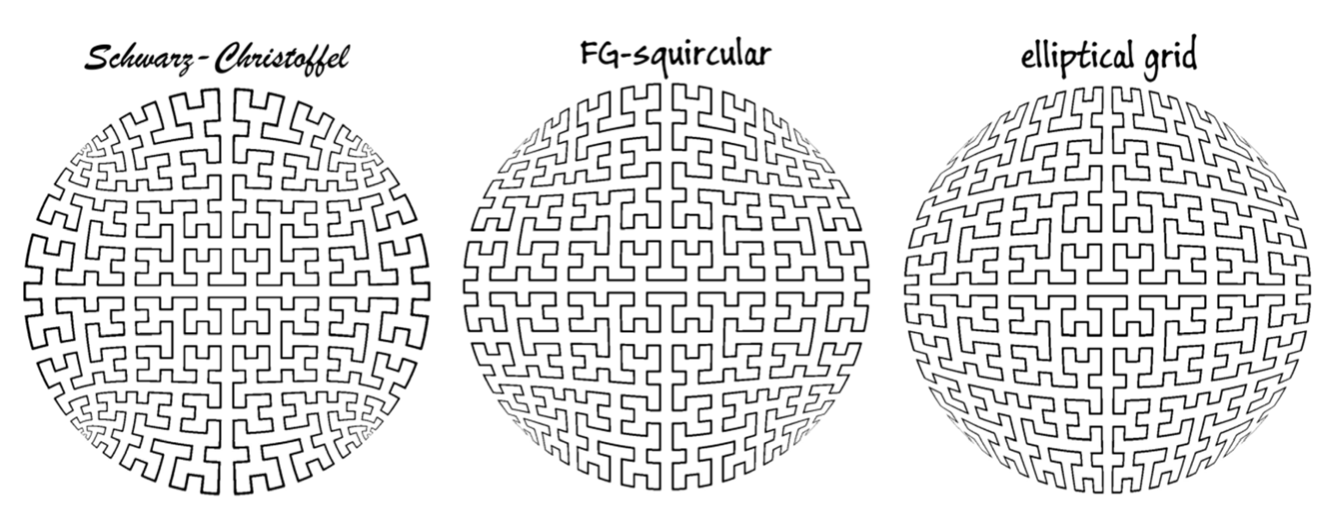
\includegraphics[width=0.8\textwidth]{fong.png}
\end{figure}

通过将方形区域映射到圆形区域的共形映射,我们可以将希尔伯特曲线共形映射到圆形区域。这种共形映射不止一个,我们可以采用任何一个。
于是得到曲线列 $H_i$ ,它可以填充圆盘。注意到这里的 $i$ 编码了一种网格的粗细,构造本身是一种不断加细的极限,这个加细过程就是通过 $i$ 来控制的。

下面的一步最为关键,我们将圆形区域视为双曲平面,这样我们就得到了一种在双曲平面上的填充方法,这个填充方法引入了一个几何的彼此垂直的线的框架,依仗这个框架,我们可以讨论运动。

\begin{figure}[ht]
\centering
\begin{tabular}{c}
\begin{tikzpicture}
  \draw (0, 0) node[inner sep=0] {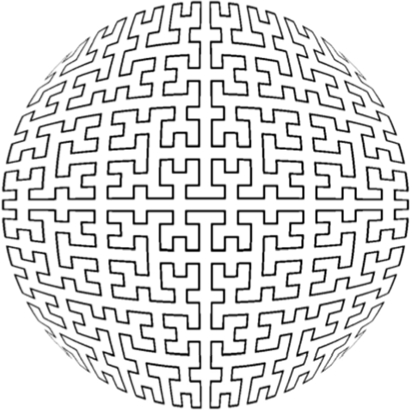
\includegraphics[width=0.8\textwidth]{crossing.png}};
  \draw[purple, thick=2.5] (0.3,0.5) .. controls (1.3,0) and (2.8,0) .. (1.8,1) .. controls (1.3,1.5) and (2.8,1) ..
                (3.3,2) .. controls (3.8,2.5) and (0.5,3.4) ..
                (-0.7,2.5) .. controls (-2.2,1.5) .. cycle;
\end{tikzpicture}
\end{tabular}
\end{figure}

对于单位圆盘内给定的简单闭区域 $D$,我们可以讨论 $D$ 的边界与上述框架的交点。注意到上述框架的边可以完美分成两类,一类是横向边,另一类是纵向边,所以交叉点也可以分为横纵两类。

我们设定一个双曲空间内全局恒定的移动速度 $v$,对于给定的粗细程度 $i$,我们可以讨论 $D$ 上的一种运动:
\begin{itemize}
	\item 基于 $D$ ,我们可以决定所有横向交叉点,然后将它们沿着交点所在的纵向线向 $D$ 外移动,保持初始交叉角度不变,同时维持双曲空间内全局恒定移动速度 $v$,移动持续一个单位时间后,我们得到一个新的区域 $D_1$ 。
	\item 基于 $D_1$ ,我们可以决定所有纵向交叉点,然后将它们沿着交点所在的横向线向 $D$ 外移动,保持初始交叉角度不变,同时维持双曲空间内全局恒定移动速度 $v$,移动持续一个单位时间后,我们得到一个新的区域 $D_2$ 。
	\item 重复上述过程,我们得到一个区域列 $D_i$。
\end{itemize}

我们的直觉是当网格无限精细时,这个运动的极限情况,它定义了一个保角的变换。

【牛顿】

你的想法具有几何证明的风味。你需要注意的一个方向是极限情况如何发挥作用。就像在微积分中,我们推理关于无穷小量的行为,你的提议也处理极限下的无穷小变换。如果这个极限转化为一个共形映射,那将非常有趣。

你必须确保网格细化不影响变换的共形性,且映射保持角度并避免扭曲。还要注意双曲空间中极限的性质 - 各向同性可能不像在欧几里得空间中那样直接。

弄清楚如何为你设想的极限过程建立严谨的数学基础。这个概念,虽然视觉上很吸引人,但需要有坚实的数学理论作为支撑。

【黎曼】

我尊重你的创新思维。你试图调和离散与连续,有限与无限,几何与分析。

关于你的方法,注意到黎曼映射定理的一个关键成分是所有在一个区域上的单射全纯函数的族的紧致性,这是 Montel 定理的一个结果。将这个应用到你的设置,它可以让你挑选出你正在描述的曲线的一个子序列,这个子序列将一致收敛到一个单射函数。

然而,挑战在于确保当网格的精细度趋于无穷大时,极限映射确实是共形的。当网格的精细度改变时,可能会有扭曲的问题。这些是你需要解决的细节,以产生一个严格工作的证明。旅程虽长,但令人兴奋。我祝你在你的探索中一切顺利。

\backmatter
\end{document}